\documentclass[a4paper]{article}

\usepackage{hyperref}
\usepackage{amsmath}
\usepackage[noend]{algpseudocode}
\usepackage{xcolor}
\usepackage{graphicx}
\usepackage[font={small}]{caption}
\usepackage[toc,page]{appendix}
\usepackage{dirtytalk} % Typesetting quotations
\MakeRobust{\say} % making dirtytalk not horrible

% Times font
\usepackage{mathptmx}

\renewcommand{\figurename}{\bf Figure}

\usepackage{geometry} % Change page margins on the fly

% Manual indents in pseudocode
\newlength\myindent
\setlength\myindent{2em}
\newcommand{\IndState}[1][1]{\State\hspace{#1\myindent}}

\usepackage[style=ieee]{biblatex}
\addbibresource{AdaptiveBarbershop.bib}

\title{An Adaptive Just Intonation Algorithm for Barbershop Music}
\author{{\bf Teun Buwalda}\\t.c.buwalda@students.uu.nl\\6787886, Utrecht University\\Bachelor's thesis}

\begin{document}

\newgeometry{top=90pt} % Temporarily decrease top margin for cover art

\begin{titlepage}

\begin{center}
	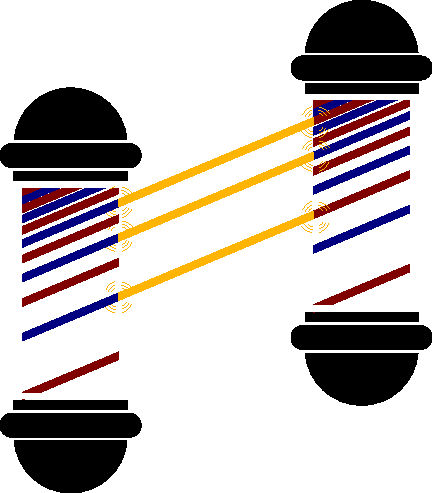
\includegraphics[height=0.3\textheight]{Figures/poles_logo.pdf}
\end{center}

\vspace{-15pt}

{
	\let\newpage\relax
	\maketitle
}

\begin{abstract}
	When harmonies in music are tuned to follow just intonation intervals, it is impossible to always keep held notes at the same pitch while also maintaining a steady tonal centre. Adaptive tuning systems make specific choices to optimise those constraints, but none have been made to specifically work for barbershop music. The first part of this thesis distils an algorithm from the tuning conventions of barbershop, optimising for the choices that need to be made for this task. The second part implements this algorithm in C$\sharp$ as a program that takes a manually tagged barbershop score as input and outputs a MIDI file with pitch bend messages. The proposed system provides just intonation at each moment in time and furthermore optimises three parameterised constraints: close-to-equal-temperament intervals in the lead voice, minimal retuning of held notes and minimal tonal centre drift. Results show that the algorithm performs well on example songs and the provided parameters have a significant effect on the resulting tuning. All code is publicly available on \href{https://GitHub.com/teuncb/AdaptiveBarbershop}{GitHub}.
\end{abstract}

\begin{quotation}
	\begin{center}
		\textbf{\textit{Acknowledgements}}
	\end{center}
	{\small \it Thank you to Jeroen Fokker and Peter van Kranenburg for their guidance throughout the project; to Jos Mulkens for his continuous support and wise thoughts; to Tijs Krammer for setting me on the course of an adaptive tuning system; to Jasper de Gier and Jay Dougherty for their expertise from the barbershop world; to Noelia Iranzo Ribera for the support group; to Than van Nispen and Marc Groenewegen for their artistic input; to Titus Mars and Jeanne Buwalda for their critical view.}
\end{quotation}

\end{titlepage}

\newgeometry{} % Reset margins for second page onward

\tableofcontents

\newpage

\section{Introduction}
\subsection{Adaptive Just Intonation for Barbershop}
The piano is out of tune. In many musical contexts, \textit{just intonation} is seen as the ideal tuning method, in which distances between tones follow simple mathematical frequency ratios. \cite{boyden_prelleur_1951, fonville_ben_1991} At the same time, western music theory recognises twelve tones per octave. \cite{persichetti_twentieth-century_1961} Sadly, tuning those twelve tones to fixed pitches such that they all follow just intonation is mathematically impossible. (\ref{intro_ji}) The modern piano, and most modern music with it, therefore use a system called \textit{equal temperament}, which only vaguely approximates the frequency ratios from just intonation. \cite{van_de_craats_fis_1989}

Music groups that have the possibility to, can attempt to alter their intonation based on the playing chord, to still achieve just intonation. \textit{Barbershop} (\ref{intro_bs}) is a genre of four-part music primarily sung in quartets, who explicitly try to achieve just intonation on every chord. \cite{barbershop_harmony_society_contest_2022, averill_bell_1999} \textit{Adaptive tuning systems} are algorithms that automatically tune each playing note such that they approximate just intonation. \cite{sethares_adaptive_1994} However, when a singer holds a note across multiple chords, there is no unbiased answer as to how exactly each note should be tuned. Holding the note at exactly the same pitch can either require a deviation from just intonation or an overall pitch drifting effect over time (\ref{intro_adaptive_ji}).

There has been extensive research into adaptive tuning systems. \cite{sethares_adaptive_2005} Most of this previous work takes a general approach, maximising dynamicity to work for live music, but they are not quite applicable to barbershop. For example, Hermode Tuning \cite{mohrlok_hermode_2003} and Pivotuner \cite{volkov_pivotuner_2022} are commercially available plug-ins that can retune piano music as it is being played. As a consequence, adaptive tuning systems generally do not model human choirs. In particular, an algorithm that takes the limitations of barbershop quartets into account, such as the roles of the four different voices, is not known to have been made to the author.

This thesis project will answer two separate questions. Question A concerns the solution to barbershop quartet's problem: {\it what adaptive tuning algorithm would a mathematically ideal barbershop quartet follow, given a score?} In this first part of the thesis, an adaptive tuning system for barbershop music will be proposed. It will optimise four criteria (outlined in Section \ref{methodoloy}) which are important to the genre. In order to validate the algorithm, the Results section (\ref{results}) will show how the algorithm accounts for these four criteria and where concessions need to be made in order to minimise conflicts between them.

Research question B is: {\it can we implement the tuning system from question A so that it models a mathematically ideal barbershop quartet?} This second part of the project should result in a C$\sharp$ program that, given a sequence of chords, can play them back justly tuned and following the genre's limitations, possibly serving as a suggestion for performers and allowing for high-level analysis of the algorithm's performance in Section \ref{results}.

To provide the necessary context to answer both of these questions, the following section will expand upon the subjects of just intonation, adaptive just intonation algorithms and barbershop music. The next section will describe the exact methodology and further describe the algorithm's constraints. Sections \ref{algorithm} and \ref{implementation} will answer research questions A and B, respectively. Section \ref{results} will evaluate the algorithm by analysing results such as global pitch drift and particularly hard-to-tune passages. Section \ref{discussion} will then place this research in the context of other literature about choirs, tuning and philosophy.

\subsection{Relevance to KI}
This thesis project is part of the bachelor Kunstmatige Intelligentie at Utrecht University. The Utrecht University AI programmes focus on Human-Centered Artificial Intelligence (HCAI), rather than trying to keep up with the latest innovations in machine learning algorithms. HCAI targets to understand, reproduce and if possible enhance human intelligence. \cite{utrecht_university_human-centered_2023} Modelling something specifically human such as music is inherently AI research, especially when trying to build an algorithm that is inspired by human performance, but performs better. Therefore, finding a tuning algorithm for barbershop music fits right into the HCAI focus area.

This study involves the definition of a new language to describe written music, was written as a computer science project and analysed afterwards from a philosophical perspective. All three of those sciences are important areas of HCAI.

\section{Theoretical Framework}
\subsection{Just Intonation}
\label{intro_ji}

\begin{figure}
	\centering
	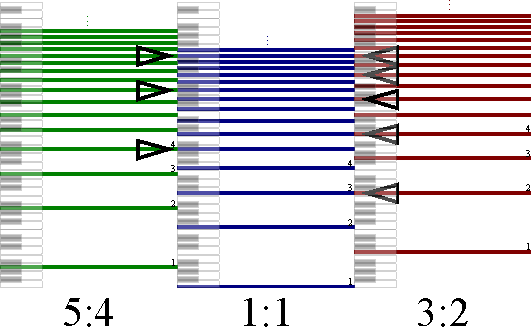
\includegraphics[height=0.35\textheight]{Figures/overtones.pdf}
	\caption{The relationship between just intonation and the overtone series, which is the cause of the \say{lock and ring} effect as pursued by barbershop musicians. The figure shows three tones with their respective overtones, the harmonic frequencies that create the sound's timbre. A piano keyboard was overlaid for pitch reference. The A (left, green) is tuned a just major third above the F (middle, blue), which makes the A's 4th, 8th and 12th overtone share the exact frequency of the F's 5th, 10th and 15th. The C (right, red) is tuned to a just fifth above the F, which means every one of its overtones which is a multiple of 2 shares its frequency with one of the F's overtones which is a multiple of 3. Because of these shared overtones, the chord has a stable sound, minimising interference by close-but-not-quite-the-same frequencies.}
	\label{fig:overtones}
\end{figure}

In many musical contexts, {\it just intonation} is seen as the ideal method for tuning. \cite{boyden_prelleur_1951} Rather than predefining each note's pitch, like necessary when tuning an instrument such as the piano, just intonation defines specific frequency ratios for each musical interval. The most common intervals are the octave (defined as $2:1$), the fifth ($3:2$) and the major third ($5:4$). For example, if an A is tuned to $220$ Hz, then an E a fifth above this A will be tuned to $220 \cdot \frac32 = 330$ Hz. The minor seventh, which is also prevalent in barbershop music \cite{barbershop_harmony_society_contest_2022}, is defined as $7:4$. \cite{van_de_craats_fis_1989} These ratios are different from the tuning system used by most modern pianos.

The ratios are drawn from the simplest intervals of the \textit{harmonic series}, which refers to the set of overtones that can be heard above nearly every sung, played or synthesised tone. When musical intervals follow these simple ratios (i.e. with a small nominator and denominator), the overtones of different tones \say{lock together} and create a specific auditory experience that many musicians strive for. This sound is caused by the fact that tones which share a simple ratio will also share many overtones (Figure \ref{fig:overtones}). Because of these shared overtones, the different tones barely interfere with each other, creating a more stable sound.

Sadly, it is mathematically impossible to devise fixed pitches for a set of twelve tones such that each pair of tones always exactly follows one of the simple ratios from just intonation. A consequence of this fact is that it is also impossible to provide a \say{perfect} tuning for the piano. This impossibility is demonstrated with the example in Figure \ref{fig:thirdsproof}, which shows two different ways to walk from a low C to a high C. Suppose we want the major third to be equal to 4 semitones, as is the case in western music theory \cite{forte_tonal_1979}, then a major third should sound between C and E, between E and G$\sharp$ and between G$\sharp$ and a high C. The major third has a ratio of $5:4$. Then the ratio between a low C and E on the piano should be $5:4$, as should the ratio between E and G$\sharp$ and the ratio between G$\sharp$ and a high C. Therefore, the ratio between the low C and G$\sharp$ should be $\frac54 \cdot \frac54 = \frac{25}{16}$ and the ratio between the low C and the high C should be $\frac{25}{16} \cdot \frac54 = \frac{125}{64}$. However, the two Cs are also one octave apart and should therefore have a ratio of $\frac21$. These two ratios are close, but not exactly the same, which shows that it is impossible to devise a tuning system such that both major thirds and octaves are always in tune according to just intonation.

\begin{figure}
	\centering
	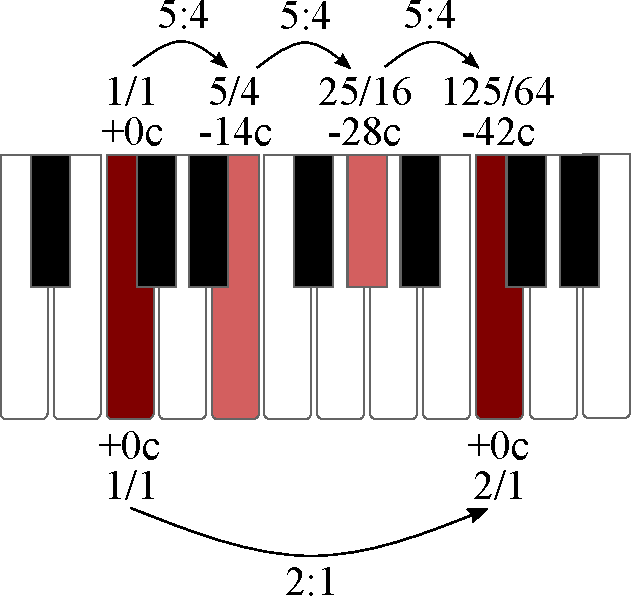
\includegraphics[height=0.35\textheight]{Figures/ThirdsProof.pdf}%[width=0.6\linewidth]
	\caption{12 fixed tones are not compatible with just intonation. For each coloured tone, its frequency ratio with the low C is written. The difference with equal temperament in cents is also written. The bottom path shows that a high C should be tuned to exactly twice the frequency of the low C when tuning the octave justly. The top path instead uses justly tuned major thirds with the standard $5:4$ ratio. The two paths come out at a different tuning for the high C, proving that major thirds and octaves are incompatible.}
	\label{fig:thirdsproof}
\end{figure}

A possible solution to the fact that just intonation is impossible to achieve with twelve fixed pitches, is to \textit{temper}, or approximate, the intervals of the harmonic series. Most modern music has accepted \textit{twelve-tone equal temperament} (often shortened to simply \say{equal temperament}) as the best substitute for just intonation. In twelve-tone equal temperament, the octave is divided into twelve logarithmically equal divisions. Since the octave is defined by the frequency ratio $2:1$, this custom puts the smallest interval (the semitone) at exactly $\sqrt[12]{2}:1$. \cite{van_de_craats_fis_1989} For example, if an A is tuned to $220$ Hz, then the lowest tone above this A, a B$\flat$, will be tuned to $220\cdot \frac{\sqrt[12]{2}}{1} \approx 233.08$ Hz. Figure \ref{fig:12TET} shows the standard tuning in equal temperament for a part of the piano keyboard. Twelve-tone equal temperament works relatively well for some intervals, such as the fifth, which is only slightly too small compared to just intonation. On the contrary, intervals like the major third and the minor seventh are significantly smaller in just intonation than in equal temperament.

\begin{figure}
	\centering
	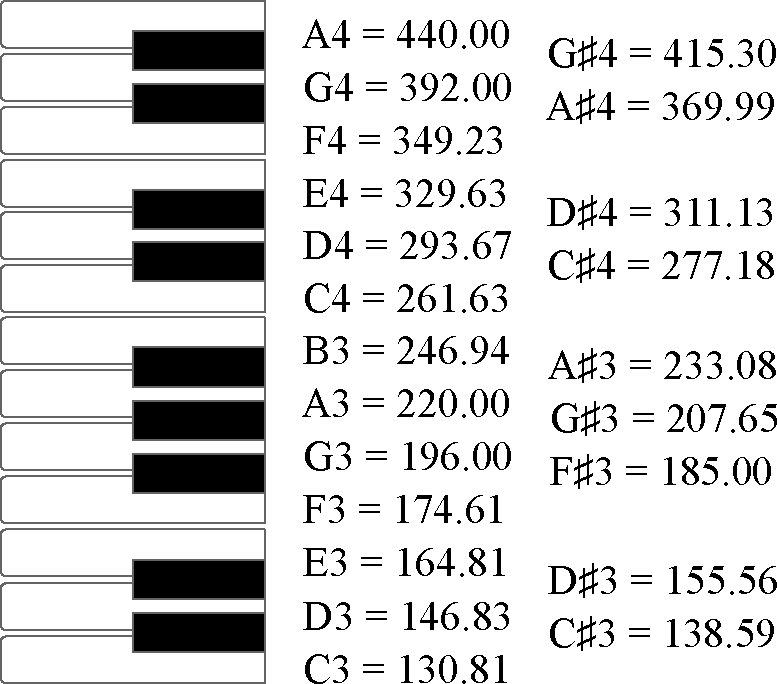
\includegraphics[height=0.35\textheight]{Figures/12TET.pdf} %[width=0.65\linewidth]
	\caption{A selection of standard frequency values for piano in equal temperament, shown in Hertz. Equal temperament is the most common tuning method and ensures that each semitone is always the same relative size, namely $\sqrt[12]{2}:1$. However, just intonation is not compatible with equal temperament; for example, if this E4 were tuned to a perfect fifth ($3:2$) with the A3 according to just intonation, it should be $330.00$ Hz, which is slightly higher than it is in equal temperament.}
	\label{fig:12TET}
\end{figure}

When talking about the difference between just intonation and 12-tone equal temperament, the \textit{cent} interval (c) is often used as a unit. 1 cent is defined as $\frac{1}{100}$ of a semitone in equal temperament, meaning it has a frequency ratio of $\sqrt[1200]{2}:1$. A justly tuned major third, for example, is 14 cents lower than a major third in equal temperament (Figure \ref{fig:thirdsproof}).

A note about terminology. The addition of the cent interval leaves us with three different ways to describe a tone's exact tuning:
\begin{itemize}
	\item as an absolute frequency in Hertz
	\item as a fraction relative to a base note
	\item as a logarithmic difference with a base note in cents.
\end{itemize}
Absolute frequencies are generally useful in physics: an A3 can be tuned to 220 Hz, whereas an E4 would be tuned to 329.63 Hz on the piano. We often use fractions to describe just intonation: when tuning an E4 to be a perfect fifth above this A3, the E4's tuning would need to be $\frac32$ times the frequency of the A3 (equivalently, 330.00 Hz). The cent interval can put this exact tuning in a musical perspective by comparing it to equal temperament: 330.00 Hz is 2 cents higher than 329.63 Hz, meaning $\frac{2}{100}$ of a semitone.

\subsection{Adaptive Just Intonation Systems}
\label{intro_adaptive_ji}
Although just intonation is impossible to achieve when all twelve piano keys have a fixed tuning, such as on an acoustic piano, it can be achieved when using instruments that can \textit{adaptively} tune specific notes. In other words, if a note's tuning is allowed to vary based on which other notes are playing, the strict mathematical ratios of just intonation can be followed. This idea is, for example, applied to ensembles with human voices, string instruments such as the violin, or trombones, since all of those instruments can continuously change their pitch. \cite{van_de_craats_fis_1989} Modern computational techniques also allow digital instruments to be tuned adaptively. \cite{sethares_adaptive_2005}

However, there is no single algorithm that completely solves the mathematical problem of just intonation. Choices need to be made with regards to optimisation of melodic intervals, held notes and tonal centre drift.
\begin{itemize}
	\item Optimisation of melodic intervals means that the intervals within the melody follow equal temperament as much as possible, making melodies sound more intuitive. \cite{dougherty_choral_2004}
	\item Optimisation of held notes means notes that keep sounding in different chords do not need to be dramatically retuned for each new chord.
	\item Tonal centre drift is a gradual lowering or heightening of the average tuning of notes, which is generally seen as undesirable. \cite{barbershop_harmony_society_contest_2022}
\end{itemize}
If held notes are allowed to retune freely, just intonation without pitch drift is possible. To achieve this goal, the performance can make sure the melody always follows equal temperament intervals and the other voices change their pitches to tune justly with the melody. \cite{dougherty_choral_2004} On the contrary, the constraint of held notes staying at the same pitch between different chords causes problems in tonal centre drift.

To illustrate this incompatibility of the held notes constraint with the other constraint, consider the scenario in Figure \ref{fig:ties_vs_ji}. In this scenario, some notes are held over changing chords. The initial C-E third requires the E to be tuned 14 cents lower in order to create the just $5:4$ ratio. Because this E is held into the next chord, the other notes need to be tuned even lower. Eventually, these held notes cause the last C to be tuned 31 cents lower than the initial one. Also, because of the different functions of the last two Es, an audible pitch shift needs to be made between them. The overall tonal centre has moved 31 cents downwards, (\textit{flat}). This downward shift shows that held notes and tonal centre drift cannot both be optimised at the same time. As another example, the music in Figure \ref{fig:input} is an adapted version of a famously \say{rising} piece of music, developed by music theorist Benedetti (1530-1590). \cite{devaney_study_2012}

\begin{figure}
	\centering
	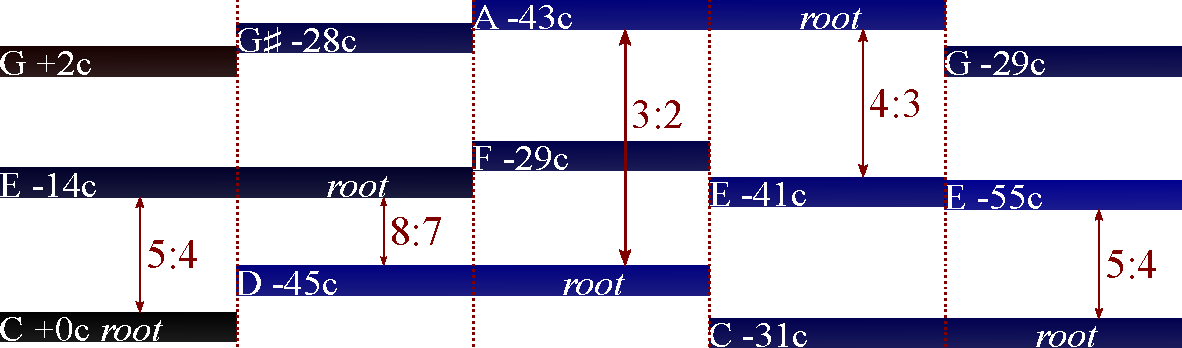
\includegraphics[width=\linewidth]{Figures/ties_vs_ji.pdf}
	\caption{Incompatibility between the just intonation, tie and drift constraints. Each note shows its note name and deviation from equal temperament in cents. The just intonation fraction is also shown for some intervals. The held notes in combination with just intonation intervals require the overall tonal centre to shift downwards.}
	\label{fig:ties_vs_ji}
\end{figure}

Much research has been done into automatic \textit{adaptive tuning systems}: computer programs that take sets of musical notes as input, and return their respective tunings according to just intonation as output. \cite{sethares_adaptive_2005} Sethares \cite{sethares_adaptive_1994} approached the problem very generally by minimising a loss function based on a sound's dissonance curve. Løberg \cite{code_grovenmax_2002} implemented a dynamic tuning system by the Norwegian composer Eivind Groven that dynamically chooses between 36 available tones to get just intervals. Schwär et al \cite{schwar_differentiable_2021} developed a loss function for intonation in order to define it as a cost minimisation problem. Horner and Ayers \cite{horner_common_1996} developed a genetic algorithm for tuning that also optimises for held notes. Commercial software such as Hermode Tuning \cite{mohrlok_hermode_2003} and Pivotuner \cite{volkov_pivotuner_2022} can be integrated into music software to retune all played notes based on the sounding chord. Hermode sums the deviations in cents from equal temperament of all sounding notes and ensures that the result is mostly equal to 0. \cite{mohrlok_hermode_2003} Conversely, Pivotuner picks a single note in each chord that should remain at the same pitch, enabling an artistic use of the resulting tonal centre drift. \cite{volkov_pivotuner_2022}

Most of the above-mentioned just intonation algorithms follow a general strategy for tuning, to apply to all genres of music. An algorithm that takes the specific properties of barbershop quartets into account, such as the roles of the four different voices, is not known to have been made to the author.

\subsection{Barbershop Music}
\label{intro_bs}
% barbershop in 1 alinea
% barbershop en just intonation
% de barbershopregels die just intonation moeilijker maken
Barbershop is a distinct genre of four-part singing that is most prevalent in North America that is primarily sung in quartets. \cite{garnett_ethics_1999} The Barbershop style is very specifically defined and has an active community that aims to preserve the genre according to its general definition. Some of the largest central events where Barbershop enthusiasts gather are competitions, where quartets are judged according to this specific definition. In this thesis, the Barbershop Harmony Society's definition of barbershop music and its Contest and Judging Handbook \cite{barbershop_harmony_society_contest_2022} will often be cited as the main source of information about priorities within the genre.

In this official definition, barbershop music is described as having four voices: tenor, lead, baritone and bass. The lead generally sings the melody, but exceptions can occur within a song. The melody is accompanied by mostly homorhythmic (i.e. in the same rhythm as the lead) harmonies in the other three voices. Chords generally do not get too complicated: most songs revolve around major and minor chords without many harmonic extensions. \cite{barbershop_harmony_society_contest_2022} Additionally, the dominant seventh chord is often described as the most important chord in barbershop music. \cite{averill_bell_1999}

The Contest and Judging Handbook (page 7-2, paragraph II.A.) \cite{barbershop_harmony_society_contest_2022} describes just intonation as one of the key elements of barbershop music. It prescribes tuning in barbershop music as follows:
\begin{quote}
	Barbershop singers adjust pitches to achieve perfectly tuned chords, and yet sing a melodic line that remains true to the tonal center. Barbershop singers strive for more precise tuning than is possible with the fixed 12-tones- per-octave of the equally tempered scale of fixed-pitched instruments, such as the piano. Essentially, we use just intonation for harmonic tuning while remaining true to the established tonal center.
\end{quote}
Barbershop singers try to minimise \say{beats} in the sound of their harmonies, the auditory artefacts that appear when chords are not tuned justly. When quartets follow interval ratios as described in Paragraph \ref{intro_ji}, the overtones of the different parts match and create a buzzing, unchanging auditory experience that is described as \say{lock and ring}.

However, very few barbershop quartets consistently achieve the high standard of just intonation. \cite{garnett_ethics_1999} The above quote immediately describes one of the major dilemmas that singers face when attempting to follow just intonation: tonal centre drift (see Paragraph \ref{intro_adaptive_ji}). Besides attempting to maintain a constant tonal centre, quartets may also try to have the lead follow consistent melodic intervals similar to those on the piano \cite{barbershop_harmony_society_contest_2022} and refrain from moving held notes around too much.

\begin{figure}
	\centering
	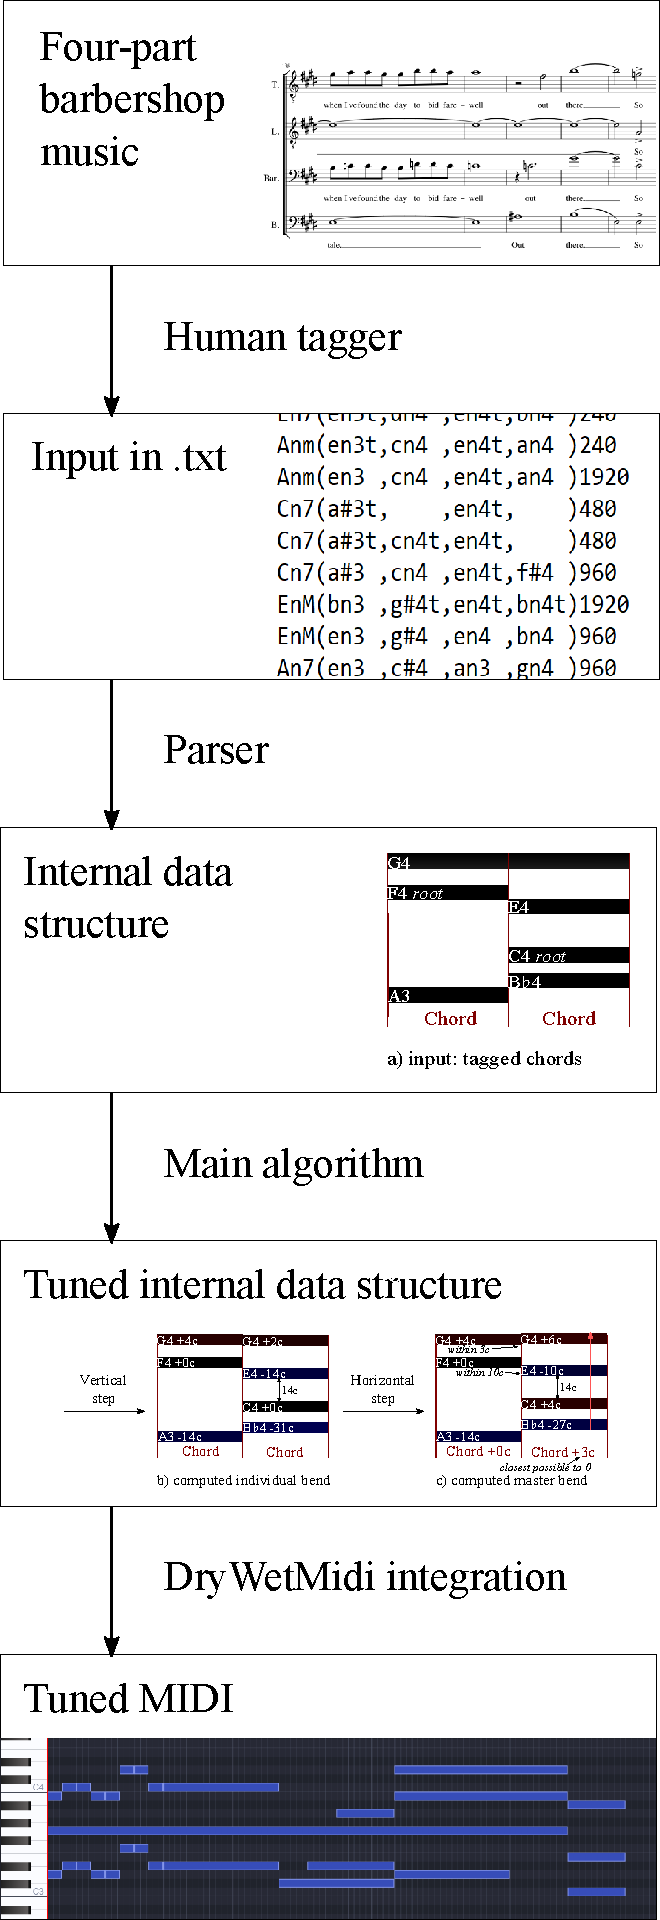
\includegraphics[height=0.8\textheight]{Figures/pipeline.pdf}
	\caption{Pipeline for the implementation of the proposed adaptive just intonation algorithm for barbershop music. The program works on any four-part score, but requires a human tagger to translate it into a language that is specific to this algorithm. A parser can then interpret this language and build the internal data structure that the main algorithm uses to determine how each note should be tuned. At last, the library DryWetMidi is used to convert the tuned internal data structure to a MIDI file with pitch bend messages.}
	\label{fig:pipeline}
\end{figure}

\section{Methodology}
\label{methodoloy}
This thesis will propose an algorithm that adaptively tunes notes in barbershop scores to just intonation. Figure \ref{fig:pipeline} shows the pipeline that the implementation should follow. The tuning system will optimise the following criteria:
\begin{enumerate}
	\item maintain just intonation on every chord [\textit{just intonation constraint}]
	\item account for the different roles of the four parts: specifically, the lead's intervals should mostly stick to those present in twelve-tone equal temperament [\textit{lead constraint}]
	\item minimise (but not necessarily eliminate) retuning of held notes [\textit{tie constraint}]
	\item minimise (but not necessarily eliminate) tonal centre drift [\textit{drift constraint}]
\end{enumerate}

The input of the algorithm is basically the score of a barbershop song. Additionally, the music is tagged with information about the intended harmonies, as those can be relevant for tuning. The output is a tuning for every note that optimises the above four constraints.

\begin{figure}
	\centering
	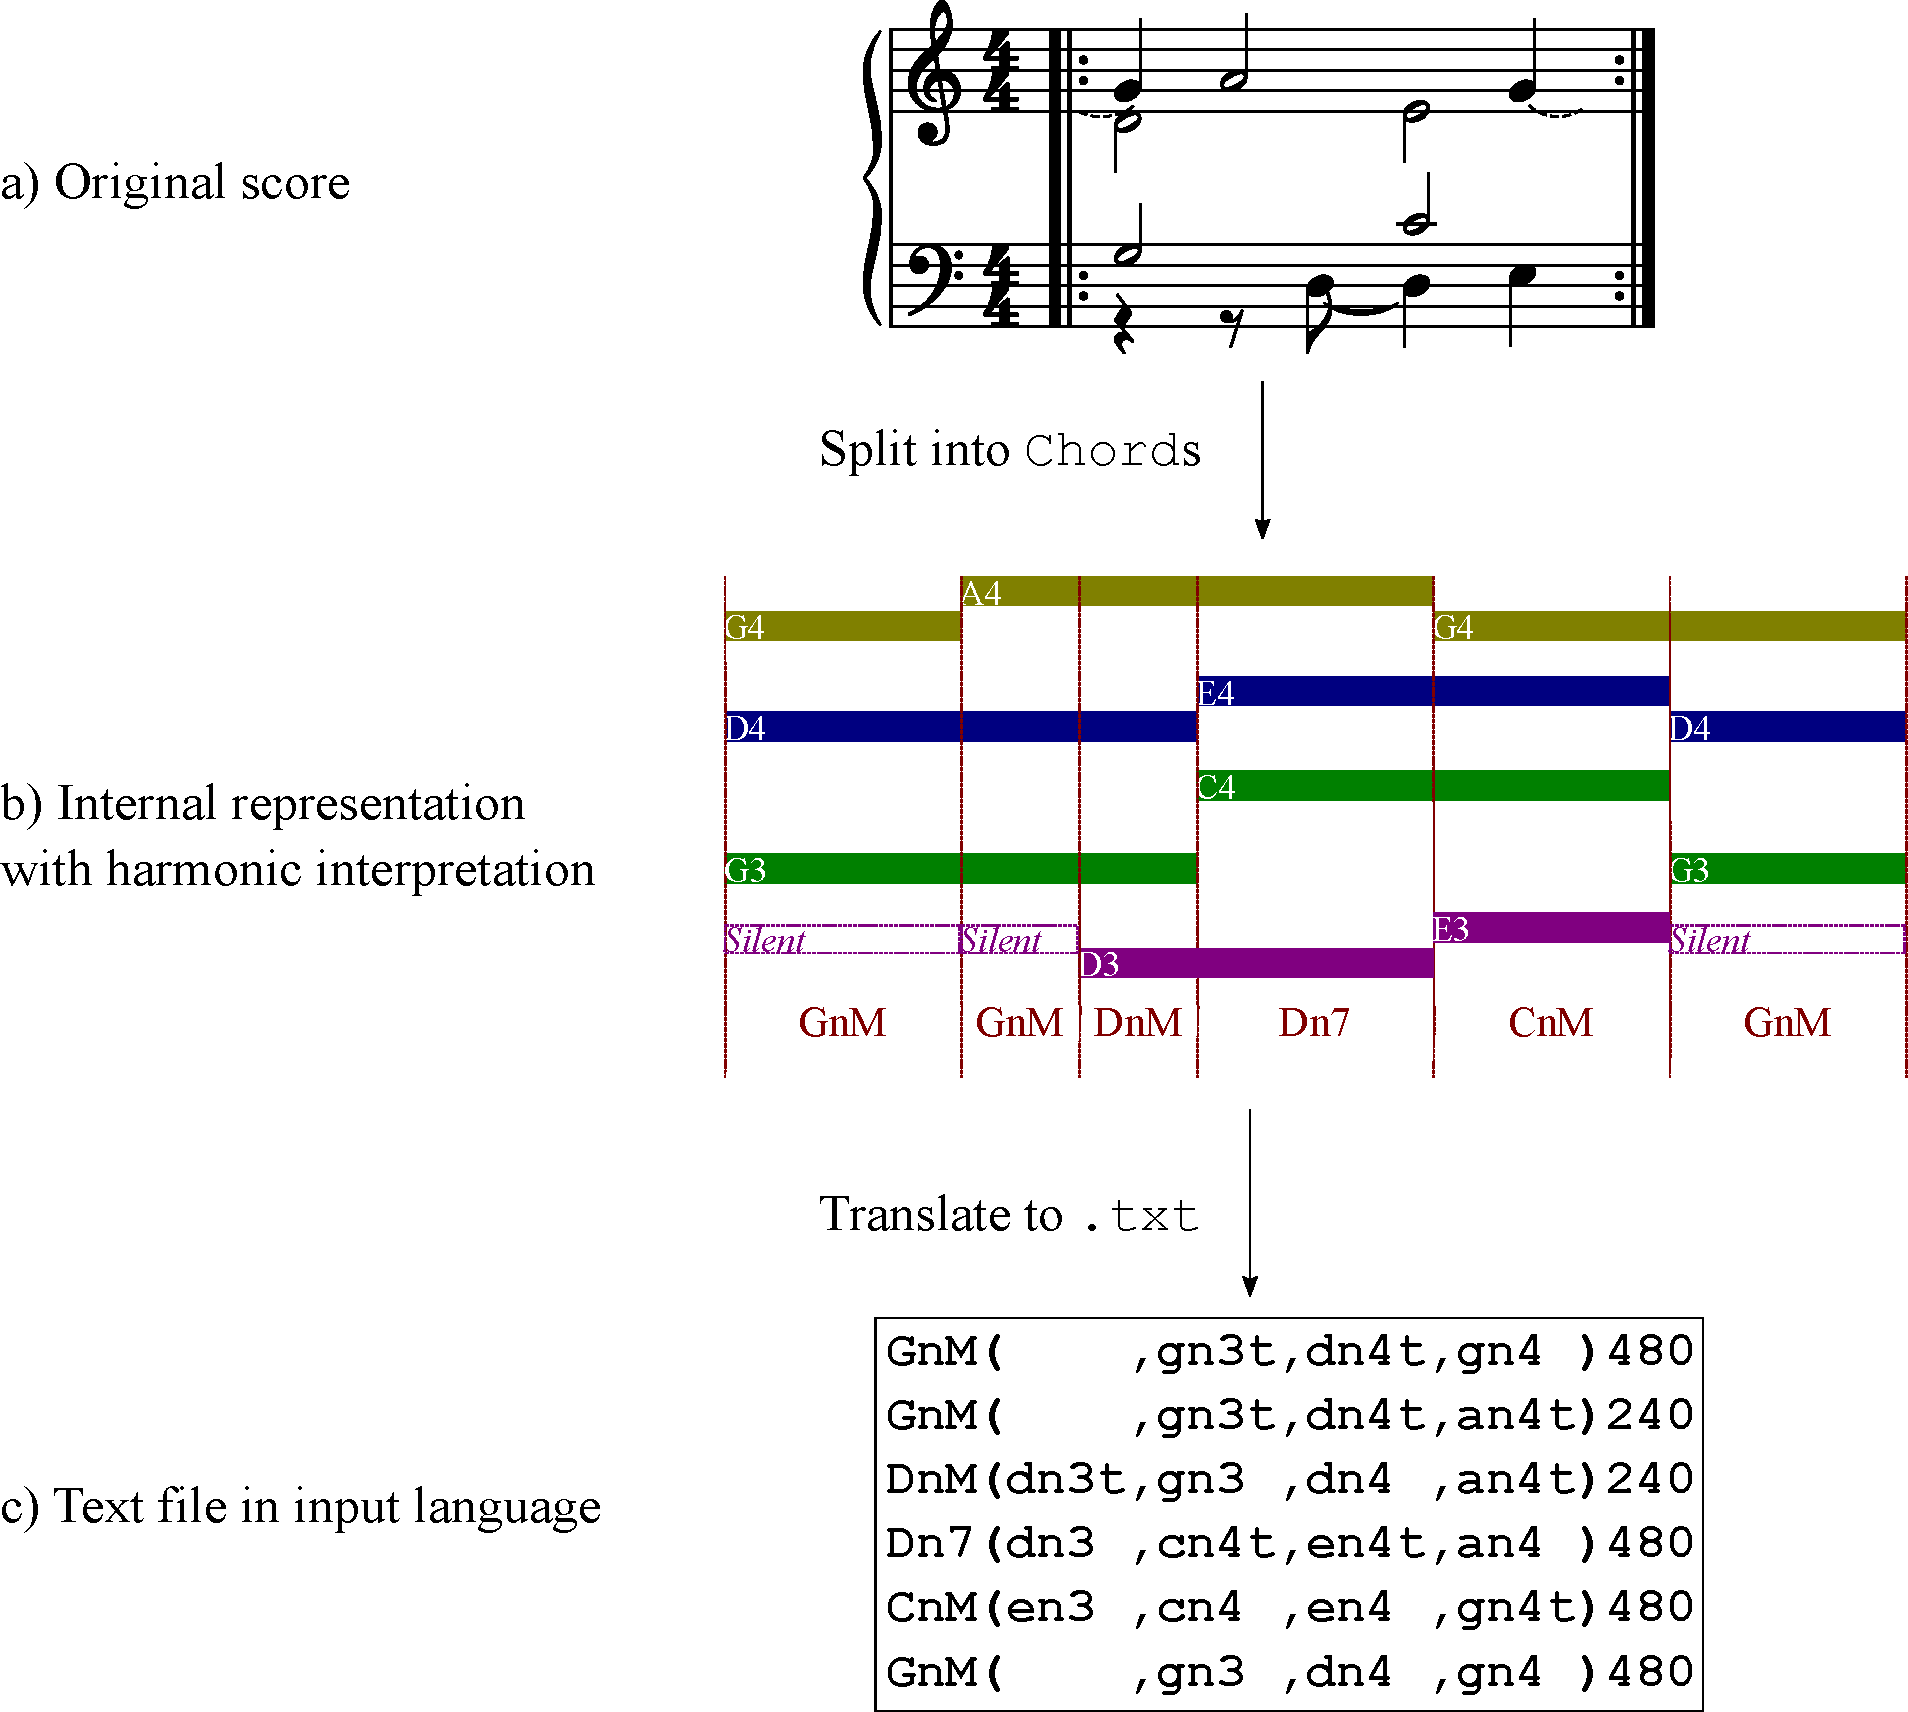
\includegraphics[height=0.35\textheight]{Figures/benedettiV.pdf}
	\caption{Example of a song in the input language. Human involvement is necessary to convert the music to the algorithm's internal data representation, especially to add chord symbols for intended harmonies.}
	\label{fig:input}
\end{figure}

For the C$\sharp$ implementation, the input already will already need to be split into a format that is friendly to the algorithm's internal representation. This representation will be different from existing digital representations of music \cite{midi_manufacturers_association_complete_2014, de_haas_music_2012, hsiao_compound_2021}, because it will already contain information that is specifically applied to this tuning algorithm. The input should therefore be written in \texttt{.txt}-files using a newly-defined language. This language is described in Appendix \ref{fig:input}. Importantly, the input splits the score into \texttt{Chord}s, which in this case are periods of time where none of the notes change. A new \texttt{Chord} begins any time one of the four voices stops singing, starts singing or moves to a different pitch. Figure \ref{fig:input} visualises such a split score. Because of this newly-defined language, a parser must be programmed to convert the input \texttt{.txt} files into the program's internal data structure. Conversion from the original sheet music to the input language is, for now, a human job.

The output of the C$\sharp$ consists of a MIDI file \cite{midi_manufacturers_association_complete_2014} and some statistics, such as how much the song had to drift in general and which chords caused the most dramatic retunings. The MIDI files mostly contain the original notes from the score, now preceded by pitch bend messages. Section \ref{implementation} will describe the MIDI conversion in further detail.


\section{Algorithm}
\label{algorithm}
% indivBend vs masterBend
% describe vertical step
% describe horizontal step
% parameters
This section will describe the tuning algorithm proposed by this thesis, thereby answering research question A: {\it what adaptive tuning algorithm would a mathematically ideal barbershop quartet follow, given a score?} The algorithm annotates each note in the song with a bend value that prescribes how much it should deviate from 12-tone equal temperament. The algorithm consists of a vertical step and a horizontal step. The vertical step satisfies the just intonation constraint from Section \ref{methodoloy}, whereas the horizontal step satisfies the other three constraints. The vertical step is a relatively standard procedure for just intonation, whereas the horizontal step is a completely new proposal. Figure \ref{fig:algo_outline} shows an outline of the full algorithm.

\begin{figure}
	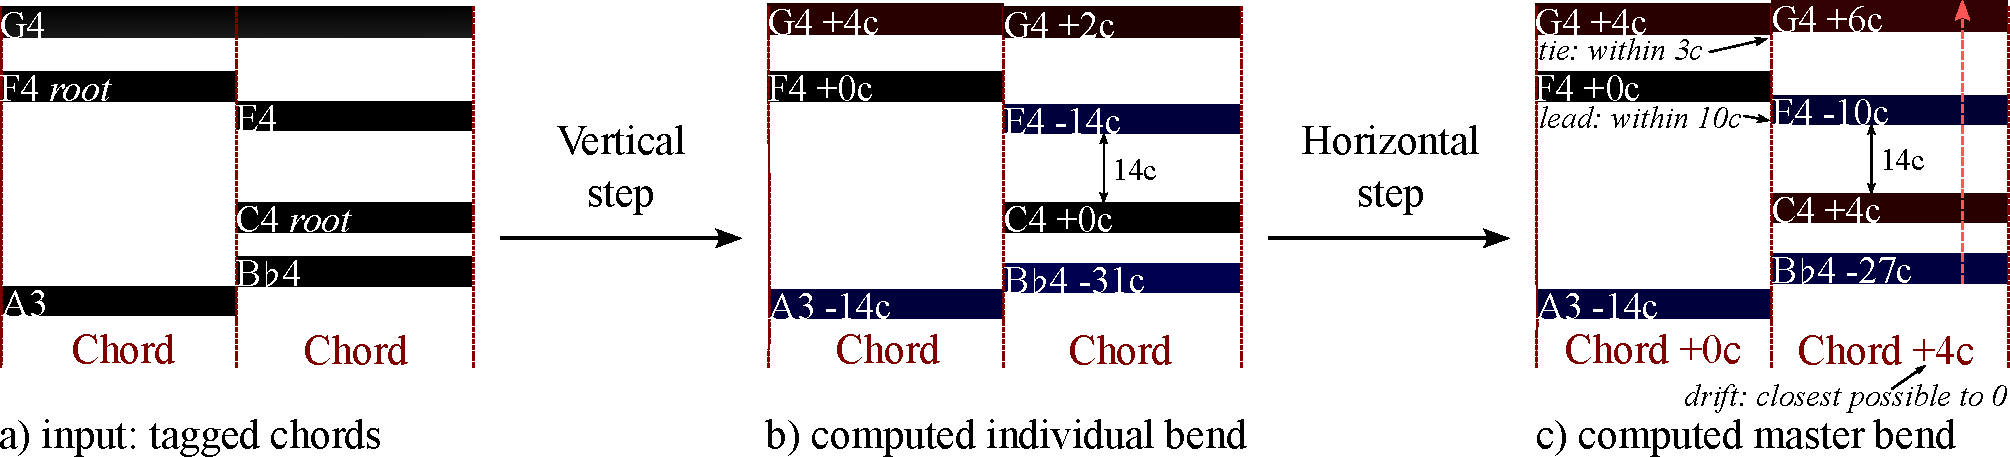
\includegraphics[width=\linewidth]{Figures/algo_outline.pdf}
	\caption{A basic view of the algorithm. tieRange = 3c, leadRange = 10c. The vertical step tunes each note separately, relatively to each other (\textit{individual bend}), satisfying the just intonation constraint. The horizontal step then attempts to satisfy the tie, lead and drift constraints by moving all notes in the chord at the same time (\textit{master bend}).}
	\label{fig:algo_outline}
\end{figure}

The algorithm distinguishes between two levels of tuning: \textit{individual bend} and \textit{master bend}. The individual bend describes how much the notes within a chord differ from each other relatively and is determined in the vertical step of the algorithm. A note's individual bend is only relative to the tuning of the other three notes in the chord, where a chord only spans a period of time where not a single note changes. The master bend, on the other hand, is used to move an entire chord's tuning up or down and is determined in the horizontal step. A note's pitch is ultimately calculated by adding its individual bend to the chord's master bend (\textit{posterior bend}) and using the result as a degree of deviation from equal temperament. Importantly, a note's individual bend never changes after the vertical step of the algorithm is done, making sure the notes of one chord always stay justly tuned with one another. Therefore, the just intonation constraint (see Section \ref{methodoloy}) is always satisfied.

The vertical step (Figure \ref{fig:algo_outline}b) determines each note's individual bend using just intonation intervals. The bend value for the chord root is always set to 0 (again, since these are relative values, that does not actually mean the root will be tuned to the regular 12-tone equal temperament value). The bend values for the other playing notes are decided using a set of interval values based on fractions relative to the chord root (Figure \ref{fig:fractions}). This set of fractions can be given by the user, but a standard set is provided. The fractions are taken from simple ratios in the harmonic series. For example, the dominant seventh chord is usually described with a $4:5:6:7$ ratio between its chord tones. Therefore, in an A dominant seventh chord (A-C$\sharp$-E-G), the G's frequency will be tuned to be $\frac74$ times the A's frequency. On the other hand, a half-diminished chord is usually described with a $5:6:7:9$ ratio, so in an A half-diminished chord (A-C-E$\flat$-G), the G will be equal to $\frac95$ times the A. Differences like this one are why the chords need to be tagged with their intended harmony.

The horizontal step (Figure \ref{fig:algo_outline}c) moves all chord notes around evenly to satisfy constraints 2-4 (lead, tie and drift; see Section \ref{methodoloy}). Specifically, it outputs a master bend value for the current chord by comparing it to the previous chord. For the lead and tie constraints, a collection of lead notes and tied notes from the previous chord is made in order to calculate how much the current master bend can move around while satisfying those constraints. Each of those notes has a desired space that the new note should move into. To illustrate: in the figure, $\mathit{tieRange}$ is set to 3 and the previous G4 is tied over, so the current G4 should be within 3 cents of the old G4. Meanwhile, $\mathit{leadRange}$ is set to 10 and the previous F4 has a posterior bend of 0 cents, so the current E4 should deviate less than 10 cents from equal temperament. After the collection of lead and tied notes has been completely run through, the algorithm chooses a value for the master bend that is as close to 0 as possible. This last step helps the drift constraint, because a master bend value of 0 means that there is no tonal centre drift.

Ultimately, the algorithm's results depend on a set of parameters given by the user. The first is a set of lists of fractions that should be used for the vertical step (Figure \ref{fig:fractions}). This first parameter is important to note, because opinions vary as to which exact tunings are the best for each interval. The other three parameters are referred to as $\mathit{priority}$, $\mathit{tieRange}$ and $\mathit{leadRange}$. $\mathit{priority}$ is either \say{lead} or \say{tie} and determines whether the lead or tie constraint should be satisfied first. $\mathit{tieRange}$, given in a unit similar to cents, determines how much a tied note is allowed to be retuned compared to its predecessor. $\mathit{leadRange}$ is similar: it determines by how many cents an interval in the lead voice is allowed to deviate from a relative interval in equal temperament (i.e. from a multiple of 100 cents). For instance, if $\mathit{tieRange}$ is set to 3 and $\mathit{priority}$ is set to \say{tie}, the horizontal step will prioritise moving the most important tied note less than 3 cents up or down over the other tied notes, the lead constraint and the drift constraint.

\begin{figure}
	\centering
	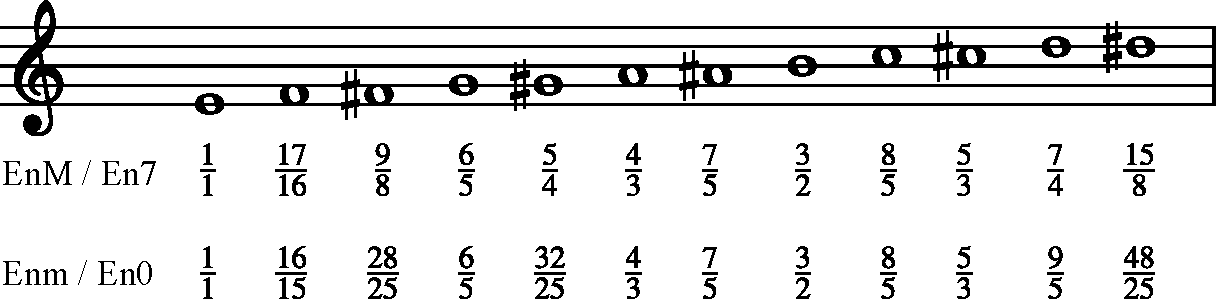
\includegraphics[width=\textwidth]{Figures/fractions.pdf}
	\caption{Different interval ratios for different chord symbols with the same root. The fractions are intervals in just intonation relative to the root note, the E. The intervals for major/dominant chords are chosen such that a dominant seventh chord follows the preferred ratio of $4:5:6:7$. \cite{van_de_craats_fis_1989} The fractions for the minor/half-diminished chords, on the other hand, are chosen such that a half-diminished chord follows $5:6:7:9$ and a minor seventh chord follows $10:12:15:18$. \cite{van_de_craats_fis_1989} These fractions are the default ones used by the vertical step of the algorithm, but can be changed using the language described in Appendix \ref{input_fractions}.}
	\label{fig:fractions}
\end{figure}

\section{C$\sharp$ Implementation}
\label{implementation}
Now that Section \ref{algorithm} has described the just intonation algorithm for barbershop music, we can look at how the algorithm was implemented into the programming language C$\sharp$. This section therefore answers research question B: {\it can we implement the tuning system from question A so that it models a mathematically ideal barbershop quartet?} The result of this section is a C$\sharp$ program that takes a song as a \texttt{.txt} file written in the language defined in Appendix \ref{input_songs} as input and outputs a MIDI file which represents the same songs, now with added pitch bend information. All code can be found on this thesis' \href{https://GitHub.com/teuncb/AdaptiveBarbershop}{GitHub repository}.

The implementation consists of five classes: \texttt{Note}, \texttt{Chord}, \texttt{Song}, \texttt{BSTuner} and \texttt{Program}. Additionally, two new structs are essential to the algorithm's workings: \texttt{Fraction} (vertical step) and \texttt{Range} (horizontal step). \texttt{Note}, \texttt{Chord} and \texttt{Song} together form the internal representation of a Barbershop song. A \texttt{Song} contains an array of \texttt{Chord}s, which in turn contains an array of exactly four \texttt{Note}s - if a part is silent in a \texttt{Chord}, its \texttt{Note}'s \texttt{playing} property is simply set to \texttt{false}. \texttt{BSTuner} contains the core of the algorithm and operates on a \texttt{Song} to tune the notes it contains. \texttt{Program} contains the \texttt{Main} method and serves as an interface for the program.

\begin{sloppypar}
The vertical step of the algorithm is basically carried out by \texttt{BSTuner.SetIndivBends} and \texttt{BSTuner.GetIndivBend}, which set the \texttt{indivBend} property for each \texttt{Note} in a \texttt{Chord}. This \texttt{indivBend} property never changes again, meaning the logarithmic distance between the chord notes remains the same and therefore the just intonation constraint is always satisfied. The methods for the vertical step use the \texttt{Fraction} struct, which represents a frequency ratio as described in Paragraph \ref{intro_ji}, relative to the chord root. The \texttt{Fraction}s used by the algorithm depend on the user input of the chord and chord type; Appendix \ref{input_fractions} describes how the desired intervals can be described. The exact frequency ratios to use can be determined by the user in \texttt{.txt} files, as described in Appendix \ref{input_fractions}.

The horizontal step of the algorithm is basically carried out by \texttt{BSTuner.SetMasterBend}, which sets the \texttt{masterBend} property for a \texttt{Chord}. The input for this method includes the $\mathit{tieRange}$, $\mathit{leadRange}$ and $\mathit{priority}$ parameters. $\mathit{tieRange}$ and $\mathit{leadRange}$ represent how \say{out of tune} the new intervals can be while satisfying the tie and lead constraints, respectively. $\mathit{priority}$ prescribes which of the two constraints should be satisfied first. To achieve this optimisation of constraints, \texttt{SetMasterBend} uses the \texttt{Range} struct, which represents a range of bend values (represented logarithmically, in equal temperament semitones). \texttt{Range}s are used to find a \texttt{masterBend} that satisfies the lead, tie and drift constraints for this \texttt{Chord}.
\end{sloppypar}

Pseudocode for the horizontal step can be found in Figure \ref{fig:pseudocodeH}. The master bend method intersects ranges with each other until no overlap can be found. If all ranges overlap, \texttt{masterBend} can be set to the closest number to 0, meaning the amount of tonal centre drift has been minimised while all other constraints are satisfied as well. If one note's range does not overlap with the current range, the function ends by returning a \texttt{masterBend} within the current range that is closest to the unsatisfiable range, ignoring the drift constraint.

\begin{figure}
	\begin{algorithmic}[1]
		\Procedure{SetMasterBend}{$\mathit{MB}_{i-1}, \mathit{Notes}_{i-1}, \mathit{Notes}_i, \mathit{tieRange}, \mathit{leadRange}, \mathit{priority}$}
		\State $\mathit{ties} \gets [$all notes in $\mathit{Notes}_{i-1}$ that have the tie property, ordered lead-bass-tenor-baritone$]$
		
		\State $\mathit{ranges} \gets [$an empty list of ranges$]$
		\State {\bf in order of} $\mathit{priority}$:
		
		\IndState $\mathit{ranges}.Add[$for all $\mathit{ties}$, the range $\mathit{MB}_i$ could move into for them to stay in their $\mathit{tieRange}]$
		\IndState $\mathit{ranges.Add}($the range in which $\mathit{MB}_i$ could move according to $\mathit{leadRange})$
		
		\If{0 is within $\bigcap \mathit{ranges}$}
		\State\Return{$\mathit{MB}_i \gets 0$}
		\Else
		\State $\mathit{currRange} \gets \mathit{ranges}$[0]
		\ForAll{$\mathit{range} \; r \; in \;  \mathit{ranges}$[1:]}
		\State $\mathit{overlap} \gets r \cap \mathit{currRange}$
		\If{$\mathit{overlap} == \emptyset$}
		\State \Return{$\mathit{MB}_i \gets$ the number closest to $r$ within $\mathit{currRange}$}
		\Else
		\State $\mathit{currRange} \gets \mathit{overlap}$
		\EndIf
		\EndFor
		
		\State\Return{$\mathit{MB}_i \gets$ the number closest to 0 within $\mathit{currRange}$}
		\EndIf
		\EndProcedure
	\end{algorithmic}
	\caption{Pseudocode for the horizontal step. The input is two Chords, both of which contain four notes. The output is a master bend value for the current chord which takes the tie, lead and drift constraints into account. $\mathit{MB}_i$ refers to the master bend of chord $i$, relative to equal temperament. The just intonation constraint has already been completely satisfied by the vertical step and does not change in this method. Because this method compromises between the current range and the next range once no overlap can be found, the drift constraint (see Section \ref{methodoloy}) may be ignored if other constraints are not compatible with each other.}
	\label{fig:pseudocodeH}
\end{figure}

After the entire \texttt{Song} has been tuned, \texttt{Song.MIDISong} and \texttt{Song.WriteMidiFile} create a MIDI file out of it using the DryWetMidi library \cite{dobroselsky_melanchalldrywetmidi_2023}. Each voice gets its own channel, meaning pitch bend messages only apply to a single voice. Every single \texttt{Chord} gets four pitch bend messages. The bend value for these messages gets calculated by adding the \texttt{Note}'s \texttt{indivBend} to the \texttt{Chord}'s \texttt{masterBend}. Since MIDI bend values only go up to two semitones \cite{midi_manufacturers_association_complete_2014}, the MIDI key for a note may be changed if its bend value exceeds 2 semitones.

\section{Results}
\label{results}
% algemeen: laat zien hoe het algoritme reageert op een stukje voorbeeldmuziek. Daarbij is dus bladmuziek nodig met annotaties (MScore naar PDF exporteren, dan in Inkscape erbij tekenen). Liefst een stukje waar het dan ook echt bij moet driften voor bepaalde parameters (probeer er een paar uit en laat alles zien).
% Ik ga hier de tag van Ring-A Ding Ding voor gebruiken
% Grafieken vanuit R met effecten op parameters

% Om te zien hoe dit algoritme het doet: stukje voorbeeldmuziek met verschillende parameters
% We gebruiken dit nummer, is interessant voor deze redenen (bv. 2 lange tied noten, zoals vaak in tags)
This section will show the proposed algorithm's effect on an example score, namely the tag of \textit{Ring-a-Ding Ding}, arranged by Anthony Bartholomew. Several good recordings of this song can be found on \href{https://www.youtube.com/watch?v=G40I5JDtfjI&t=147s}{YouTube}. Figure \ref{fig:ding_sheets} shows the sheet music for this tag. \cite{dominikschaller_barbershop_2015} Since both the bass and tenor voices hold notes for a long time while the lead and baritone sing phrases in-between, \textit{Ring-a-Ding Ding} is a good example to show how the proposed algorithm makes choices in ambiguous scenarios. This thesis' \href{https://github.com/teuncb/adaptivebarbershop}{GitHub repository} also contains the algorithm's output MIDI files for \textit{Ring-a-Ding Ding}, as well as the results from other barbershop snippets, so it is possible to listen and compare.

Figure \ref{fig:results} shows the effects that the three parameters (tieRange, leadRange and priority, see \ref{algorithm}) have on the lead, tie and drift constraints in \textit{Ring-a-Ding Ding}. Note that the just intonation constraint is, because of the permanent nature of the vertical step, always satisfied. The lead constraint is quantified as the number of lead intervals that had to deviate more than 10 cents from equal temperament intervals. The tie constraint is quantified as the number of pairs of held notes where the second note was more than 3 cents higher or lower than the first. The overall tonal centre drift with these parameters has also been plotted.

% ranges ~ drift, flinke sprong nadat range de bar overschrijdt, prio niet zoveel effect (ws soms 1 noot), 
The plots show that tonal centre drift is negatively correlated with both $\mathit{Range}$ parameters: if notes and intervals are allowed to differ more from the ideal changes, then the song will drift less. Specifically, a stricter $\mathit{tieRange}$ causes less pitch drift earlier (\ref{fig:results}a, b) than a stricter $\mathit{leadRange}$ (\ref{fig:results}c, d) for this song. Since an \say{audible retuning} is set to be at least 3 cents, the number of audible retunings leaps after the $\mathit{tieRange}$ passes 3 cents. The song only needs to deviate from equal temperament in lead intervals a couple of times, which is why this leap is invisible in the red line. When the $\mathit{priority}$ is set to \say{lead} (\ref{fig:results}b, d), not a single deviation from equal temperament is necessary and the number of tied note retunings is relatively low in general.

\begin{figure}
	\centering
	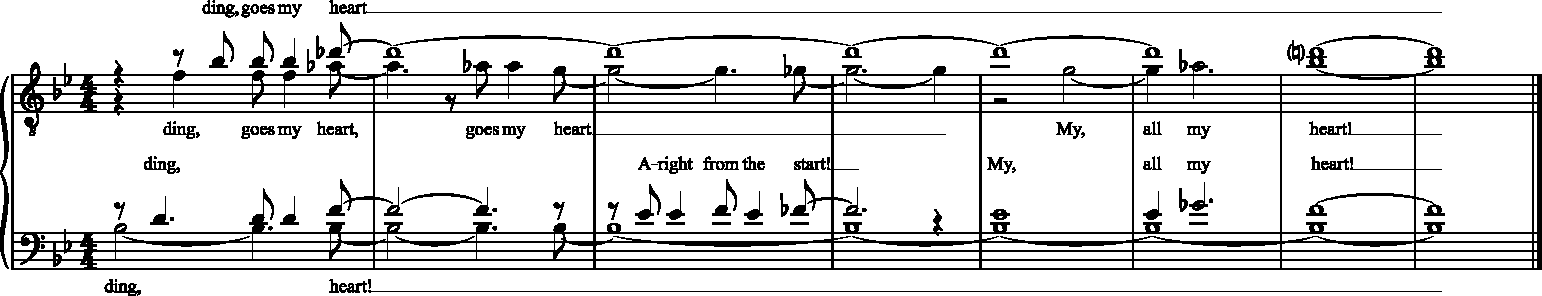
\includegraphics[width=\linewidth]{Figures/Ding_MuseScore.pdf}
	\caption{Sheet music for the tag of \textit{Ring-a-Ding Ding}, a barbershop arrangement by Anthony Bartholomew. This tag was used as an example song in the Results section.}
	\label{fig:ding_sheets}
\end{figure}

\begin{figure}
	\centering
	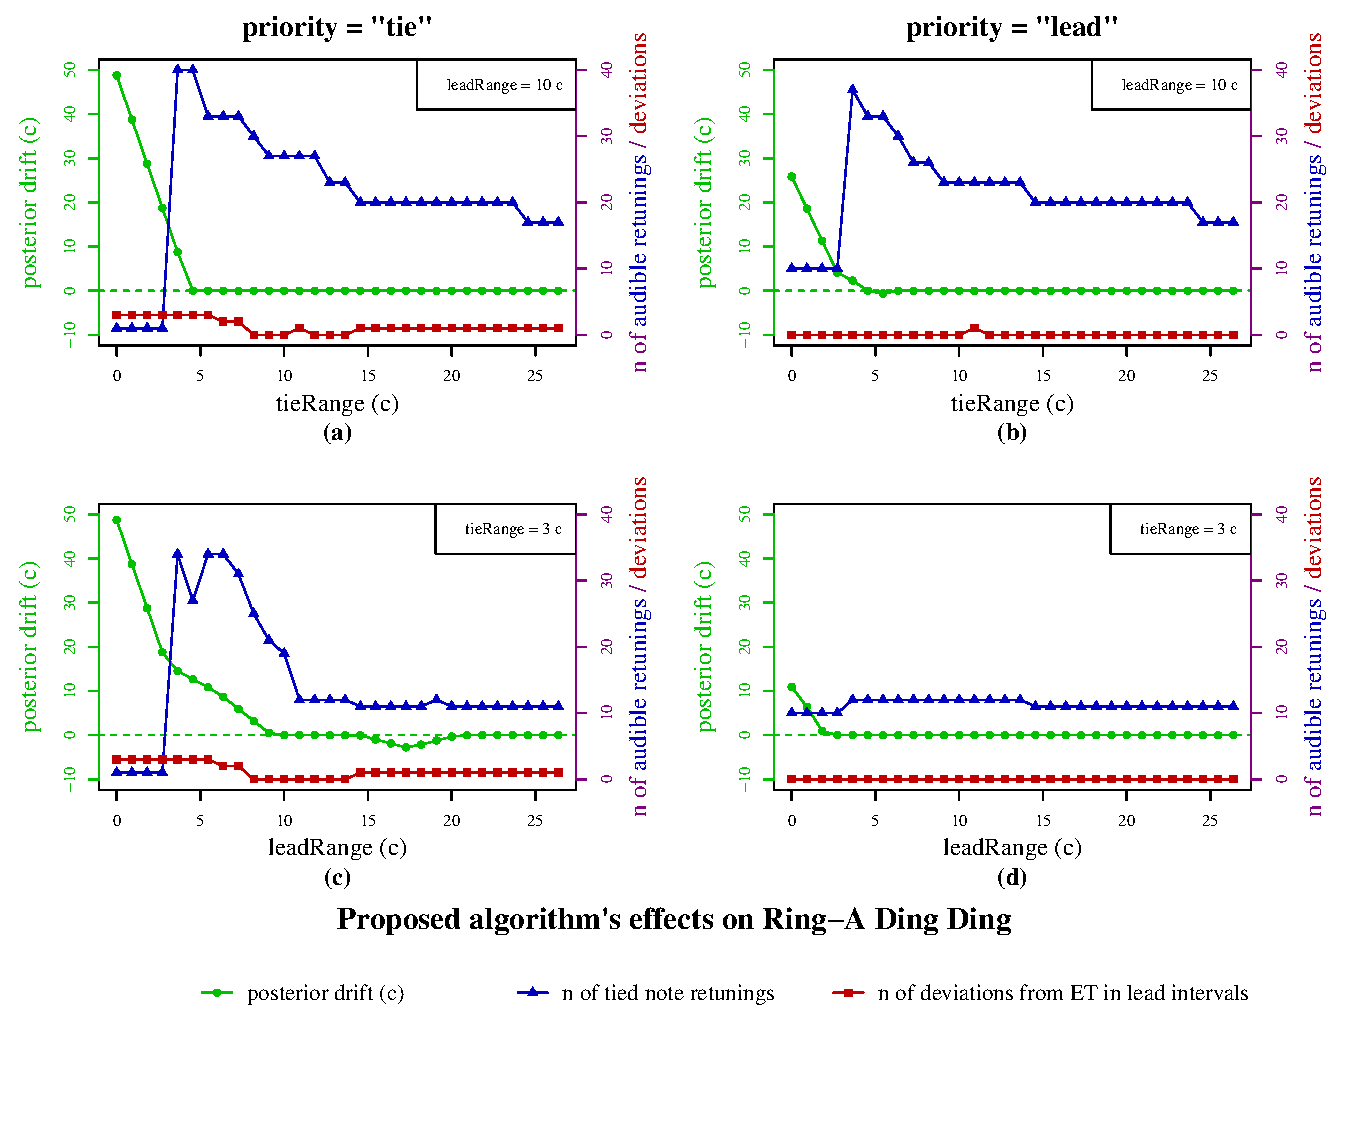
\includegraphics[width=\linewidth]{Results/effects_ring.pdf}
	\caption{Results from the proposed algorithm on the tag of \textit{Ring-a-Ding Ding} (sheet music in Figure \ref{fig:ding_sheets}). The graphs show the effects of parameter changes (x-axis) on three measures (y-axes): overall tonal centre drift in cents (green), number of tied note retunings over 3 cents (blue) and number of deviations from equal temperament in the lead voice larger than 10 cents (red). The tieRange and leadRange parameters determine how loosely the algorithm allows the most important held notes to retune (tie constraint) and how loosely it allows the lead voice's intervals to deviate from equal temperament. The left two graphs have the \textit{priority} set to \say{tie}, whereas the right two graphs have it set to \say{lead}. Both parameters appear to have a similar effect on how many notes need to retune, how many lead intervals are outside equal temperament and how much the song drifts overall.}
	\label{fig:results}
\end{figure}

\section{Discussion}
\label{discussion}
\subsection{Evaluation of Results}
% Was het goed?
% Interessant: dipje in groen bij leadRadius = 17

% Antwoord vraag A: is dit het ideale algoritme? niet per se, je kunt nadenken over tie retunings eens per maat ofzo. maar 
Research question A was: {\it what adaptive tuning algorithm would a mathematically ideal barbershop quartet follow, given a score?} In this thesis project, an algorithm was proposed as the ideal tuning system for barbershop quartets, immediately approaching an answer to this question. The results show that the proposed algorithm successfully optimises the four constraints according to given priorities. However, as expected, there is no definitive answer to question A; it is impossible to tune the \textit{Ring-a Ding Ding} tag in such a way that all four constraints from Section \ref{methodoloy} are completely satisfied. 

% Antwoord vraag B: is het succesvol geïmplementeerd? Ja!
Research question B was: {\it can we implement the tuning system from question A so that it models a mathematically ideal barbershop quartet?} The algorithm was successfully implemented in C$\sharp$, making the answer to question B a definitive yes. Of course, whether this implemented algorithm sounds like the perfect barbershop quartet is a matter of opinion. Nonetheless, since every chord is in just intonation and overall pitch drift can be kept to a minimum, it can be said that this algorithm poses a \textit{mathematically ideal} solution to the tuning problem that is implicitly posed by the Barbershop Harmony Society's Handbook. \cite{barbershop_harmony_society_contest_2022}

The results from Figure \ref{fig:results} show that completely satisfying the four constraints posed in Section \ref{methodoloy} is, as predicted, not possible with the proposed algorithm. When $\mathit{tieRange}$ and $\mathit{leadRange}$ are close to 0, the tie constraint is satisfied, but we land on a different tonal centre than we started on, meaning the drift constraint is not satisfied. With looser ranges, the drift constraint can be satisfied, but there will always be some tied notes that need to be retuned, meaning the tie constraint has to be let go. Different barbershop songs may yield different results, but the optimal setting for \textit{Ring-a-Ding Ding} appears to be $\mathit{tieRange} \approx 3\text{ c}, \mathit{leadRange} \approx 3\text{ c}, \mathit{priority} = $ \say{lead}. Because it has multiple voices with long notes, \textit{Ring-a-Ding Ding} is a relatively hard song to tune, meaning it might be possible to find a more satisfactory tuning for some common barbershop songs. Additional examples of songs can be found in this thesis' \href{https://github.com/teuncb/adaptivebarbershop}{GitHub repository}.

% Daar hoort bij: JI altijd geslaagd, lead altijd geslaagd als prioriteit lead is, twee ties tegelijk kan nog wel eens stomme resultaten opleveren
In general, the proposed algorithm tunes barbershop songs to a high degree of perfection. Note that the just intonation constraint is always the top priority of this algorithm, meaning it is not possible to compromise how much any passing chord is in tune using this algorithm. Compromises are always made by retuning tied notes, deviating from equal temperament intervals in the lead and/or drifting away from the tonal centre. The algorithm successfully proves that the just intonation, lead and drift constraints can be completely satisfied when given the priority, i.e. the red plot in Figure \ref{fig:results}d remains at zero. This algorithm does tend to have problems if more than one voice holds a tied note, since it will always completely prioritise one voice over the other. Future endeavors could choose to more equally distribute the tie constraint over the four voices, or allow held notes to retune more dramatically on certain beats.

A few interesting remarks can be made about the results from Figure \ref{fig:results}. Firstly, a very low $\mathit{tieRange}$ actually causes a very high number of retuned tied notes over 3 cents (\ref{fig:results}a, b). That is because the algorithm prioritises tied notes in the order lead-bass-tenor-baritone; if the bass and tenor are both holding a note, then the tenor note might be let go to ensure that the bass note does not need to be retuned. Therefore, if the algorithm is very strict about the bass retuning, the tenor will only need to be retuned even more. Secondly, a steady $\mathit{tieRange}$ and a $\mathit{priority}$ set to lead appears to be a simple way to get a relatively low number of tied note retunings (\ref{fig:results}d). This is because the just intonation, lead and drift constraints can always be completely satisfied if they have the priority \cite{dougherty_choral_2004}, which also means the tied notes need to compete less which each other. Lastly, when the $\mathit{priority}$ is set to \say{tie}, there is a certain area of $\mathit{tieRange}$ and $\mathit{leadRange}$ values where not a single lead interval has to deviate from equal temperament, even though both lower and higher values for the Range parameters cause some deviations to occur (\ref{fig:results}a, c). The exact reason for this dip is unclear, but it most likely also has to do with the effects of the algorithm's priorities.

\subsection{Musical Context}
% Is zo'n algoritme wel realistisch? Iets met een cognitief model
% Hagerman citaties; Bye Bye Pythagoras: is JI wel beter?
% 12-toonsstemming is niet overal het best; andere approach is Sethares
The use of an algorithm such as the one proposed is debatable. For human performers, this algorithm would be impossible to carry out; the exact calculations required would be too complicated to carry out while singing and the tiniest intonation changes cannot be replicated using the human voice. Also, the algorithm's goal is not to \say{capture theories of cognitive functioning in mathematical or computational form}, which means it is not exactly a cognitive model. \cite{van_maanen_interpretation_2021} However, the algorithm's results could serve as a reference for real singers to hear what a potentially ideal method of tuning could be. Additionally, high-level findings from the algorithm such as described in Section \ref{results} could give singers a frame of reference as to how they should generally tune their notes in a barbershop context.

Even the concept of just intonation itself is a subject of debate: are the intervals from the harmonic series really the best way to tune? Hagerman \& Sundberg \cite{hagerman_fundamental_1980} analysed recordings of barbershop quartets and found that the tenor, baritone and bass use the lead as a reference to adjust their pitches, but their intervals often deviate from just intonation. \cite{abbott_acoustic_2001} Other studies have found musical intervals so similarly deviate from just intonation. \cite{nordmark_intonation_1996, sundberg_rules_2009} Thanks to new technologies in music information retrieval, intonation and drift in choirs have been analysed in recent years. \cite{devaney_study_2012, mauch_intonation_2014, dai_intonation_2019} Results from analyses like these have even led some researchers to conclude that just intonation as a whole is not the ideal tuning method. \cite{parncutt_psychocultural_2018, kopiez_intonation_2003} However, not enough research has been done to completely isolate these findings from twelve-tone bias. \cite{burns_7_1999}

At the same time, it is important to note that twelve-tone bias does play a role in this article's proposed tuning system. Barbershop music is composed with the western standard division of the octave in mind, which means notes that sound the same on the piano are often meant to sound the same in singing as well. A tuning method that does not adhere to the twelve-tone system and is, therefore, more culturally independent, was proposed by Sethares. \cite{sethares_adaptive_1994} Instead of using fractions from the harmonic series, he proposes to analyse a note's timbre using its \textit{dissonance curve}. However, since the present article focuses specifically on barbershop, dissonance curves for voiced tones will always adhere to the natural harmonic series \cite{duifhuis_measurement_1982} and using the twelve-tone system is commonplace. For these reasons, it was decided not to use Sethares' proposal in the current research.

\subsection{Philosophical Framework}
% strong vs weak AI: wat het is, wat dit is en waarom, wat als dit het niet zou zijn
% ethics: ethical concerns of computers making music: future of work (calo), maintain the legal status of tools (fjeld), achievement gap (danaher). 
Philosophy regarding artificial intelligence recognises two classifications of views about the future of the technology: \textit{weak AI} and \textit{strong AI}. Weak AI supposes that AI can merely exist as tools to make human lives easier, whereas strong AI also allows it to learn and understand as humans do and have other cognitive states. \cite{searle_minds_1980} Since music-making is a creative process, crossing the border of outperforming humans in music might be seen as strong AI. \cite{gottschall_rise_2015} However, when a computer is only following a set of rules without being able to add emotion, it might lack the ability to create beauty. \cite{braga_emperor_2017} The fact that the proposed algorithm in this thesis only follows rules to enrich man-made music explicitly places it in the classification of weak AI.

Tools that allow computers to make music might give rise to a number of ethical concerns which are important to keep in mind during future developments. Firstly, tool-assisted art making may cause an \textit{achievement gap}, in which the connection between human effort and workplace outcome is severed, thereby undermining achievement in the workplace. \cite{danaher_automation_2021} Secondly, human control over these systems remains important. \cite{fjeld_principled_2020} The UNI Global Union prescribes that AI systems must keep the legal status of tools, meaning the responsibility stays with humans. \cite{uni_global_union_top_2017} Lastly, AI systems might take over human jobs, which might have different consequences: either humans get more rewarding tasks, or human jobs completely disappear, creating the need for a universal basic income. \cite{calo_artificial_2017}

The proposed algorithm alone is not enough to replace human barbershop quartets; its intended use is to serve performers with a suggestion of how to sing their repertoire. However, in combination with tools such as Synthesizer V \cite{hua_synthesizer_2020}, which can output a human-sounding performance given a score, an automatic tuning system does potentially bring the state-of-the-art one step closer to replacing human singers. Therefore, it is important to keep in mind achievement gaps, human control and the effect on the economy in further research.

\subsection{Future Work}
% MIDI Input of op z'n minst abc-notatie
% Analyse van echte barbershopintonatie (AMPACT, devaney)
The input for this algorithm was a newly-defined language, described in Appendix \ref{input_songs}. Translating a score into this language has turned out to be a tedious process and could be optimised better. One more common way to describe music in plain text is \textit{abc notation}, which also allows chord annotation. \cite{walshaw_abc2mtex_1997} However, since automatic chord recognition has improved in the past couple of decades \cite{burgoyne_cross-validated_2007}, an implementation of this algorithm could easily be built that simply takes MIDI as input and automatically annotates the chords. Essentially, the only thing that the tuning system has to add as output is pitch bend messages.

The scope of this thesis did not allow for a comparison to real-world barbershop quartets. In recent years, systems such as AMPACT can be used to evaluate the tuning tendencies of real choirs. \cite{devaney_study_2012, chandna_deep-learning_2022} Analysing the difference between mathematically ideal algorithms such as the one proposed and the tendencies of professional barbershop quartets could lead to an even better tuning system. Eventually, a tuning system might be developed that all barbershop musicians can refer to when singing their genre.

\subsection{Code Availability}
All code for the C$\sharp$ implementation of the algorithm, along with example songs, their MIDI output and analyses can be found on \texttt{\url{https://GitHub.com/teuncb/AdaptiveBarbershop}}.

% \bibliography{AdaptiveBarbershop.bib}
% \bibliographystyle{ieeetr}
\printbibliography
\noindent The cover art and all figures including piano keyboards were designed using assets from Freepik.com.

\begin{appendices}
These appendices describe the language in which \texttt{.txt} files should be written for the presented C$\sharp$ program to interpret music. Appendix \ref{input_songs} describes how a Barbershop score can be converted into a \texttt{.txt} file. Appendix \ref{input_fractions} then describes how a user can prescribe just intonation frequency ratios based on a playing chord.

\section{Input Language for Songs}
\label{input_songs}
% Notes: n, b and #; octaves; tied notes
% Chords: with 4 notes, sometimes not playing; chord symbols
% duration in MIDI, timecode at 480 (find unit), only used for MIDI
The C$\sharp$ implementation of the proposed algorithm takes \texttt{.txt} files containing tagged scores as input. Converting a score to a \texttt{.txt} file involves splitting it into bits of time where no notes change called \texttt{Chord}s and interpreting the playing harmonies to add chord symbols. Figure \ref{fig:input} shows an example of the translation process. Some more examples of converted scores can be found in the \href{https://github.com/teuncb/AdaptiveBarbershop/tree/main/Songs}{Songs folder on the GitHub repository}.

A note consists of exactly four characters: a note name, an accidental, an octave, and a tie indication. If a voice is silent in a \texttt{Chord}, the note should simply be four spaces. The note name is simply a lower-case letter between a and g. The accidental is a character from the set $\{\texttt{\#}, \texttt{b}, \texttt{n}\}$, which stand for \say{sharp}, \say{flat} and \say{natural}, respectively. The octave is a number between 0 and 8, written as in Scientific Pitch Notation. \cite{pollens_pitch_2022} The octave makes no difference in the tuning process, but the note must be present on an 88-key piano. The tie indication is either \say{\texttt{t}} or a space, which indicates whether this note keeps playing in the next \texttt{Chord}. For example, \say{\texttt{an3 }} would be the highest A below middle C that stops after this \texttt{Chord}, whereas \say{\texttt{e\#4t}} would be the first E$\sharp$ (or, in this case equivalently, F) above middle C, that keeps playing after this \texttt{Chord}. In the last example, the next \texttt{Chord} should also contain this E$\sharp$ or F in the same voice.

A chord symbol consists of exactly three characters: a note name, an accidental and a chord type. The note name and accidental work the same as for notes, though in a chord symbol the note name should be in upper-case. The chord type is a character from the set $\{\texttt{M}, \texttt{m}, \texttt{7}, \texttt{o}, \texttt{0}\}$, which stand for major, minor, dominant seventh, diminished and half diminished, respectively. The chord type decides which \texttt{Fraction}s file is chosen to tune the notes in the current \texttt{Chord}. The default algorithm uses the same file for major and dominant chords and also uses the same file for minor and half-diminished chords.

A \texttt{Chord} is described using a single line containing a chord symbol, four notes (enclosed by brackets and separated by commas), a duration and optional comments after a \texttt{\%}. The notes are ordered bass - baritone - lead - tenor. Like the octave, the duration is only used for MIDI output and has no effect on tuning. The algorithm always uses the standard \cite{dobrian_timing_2014} timecode of 480 ticks per quarter note, meaning an eighth note would be $0.5 \cdot 480 = 240$ ticks.

\section{Input Language for Fractions}
\label{input_fractions}
% slashes
% in code
A \texttt{.txt} file describing interval ratios consist of exactly twelve lines, one for each of the twelve possible notes in the input. Each line consists of a frequency ratio with the root and additional comments after a \texttt{\%}. The first line corresponds to the chord root and is therefore logically \texttt{1/1}. The next lines each count up from the root in semitones. The eighth line therefore corresponds to a fifth, meaning it would most likely be \texttt{3/2} (see \ref{intro_ji}). The \href{https://github.com/teuncb/AdaptiveBarbershop/tree/main/TuningTables}{TuningTables folder on the GitHub repository} contains some examples of \texttt{Fraction} files.

\end{appendices}

\end{document}